

\chapter{Referencial Teórico}
\label{chap:referencial-teorico}

\section{MLP (Perceptron Multicamadas)}

Como é mostrado na Figura \ref{fig:subfigura1}, uma Rede Neural Multicamadas (MLP – \textit{MultiLayer Perceptron})
é formada por um conjunto de neurônios, também conhecidos como
Perceptrons. Uma MLP consiste em uma camada de entrada, juntamente com uma ou mais camadas ocultas.
No processo de treinamento, é empregada uma técnica chamada retropropagação (\textit{backpropagation}), que
ocorre em duas fases distintas: a propagação para frente (\textit{forward}) e a retropropagação propriamente
dita (\textit{backward}), assim como ilustra a Figura \ref{fig:subfigura2}. Durante a propagação para frente, os dados são passados pela rede, camada por camada,
permitindo que as saídas da rede sejam calculadas. Em seguida, durante a fase de retropropagação, os
erros entre as saídas previstas e os valores reais são calculados e propagados de volta através da rede,
ajustando os pesos das conexões para minimizar esses erros. Esse processo iterativo é fundamental para o
treinamento eficaz de uma MLP, permitindo que ela aprenda e se adapte \cite{su12114776}.  

\begin{figure}[h]
    \centering
    \caption{Estrutura e atividade de uma rede MLP, imagens de \cite{su12114776}.}
    \begin{subfigure}{0.4\textwidth}
      \centering
      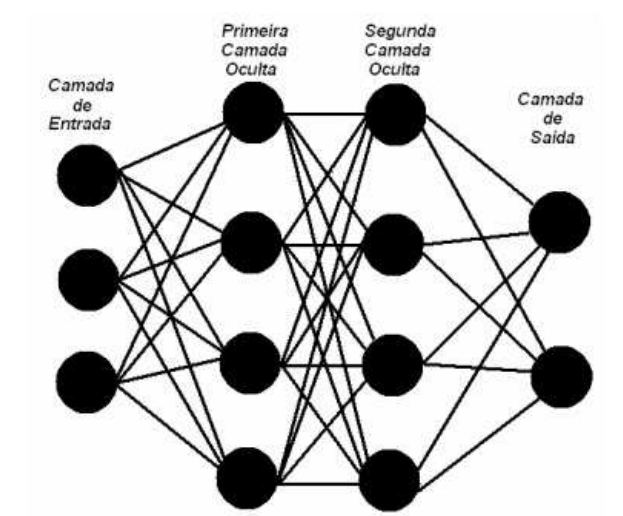
\includegraphics[width=\linewidth]{figuras/MLP/rede_MLP.png}
      \caption{Camadas de uma MLP.}
      \label{fig:subfigura1}
    \end{subfigure}
    \hspace{5mm}
    \begin{subfigure}{0.45\textwidth}
      \centering
      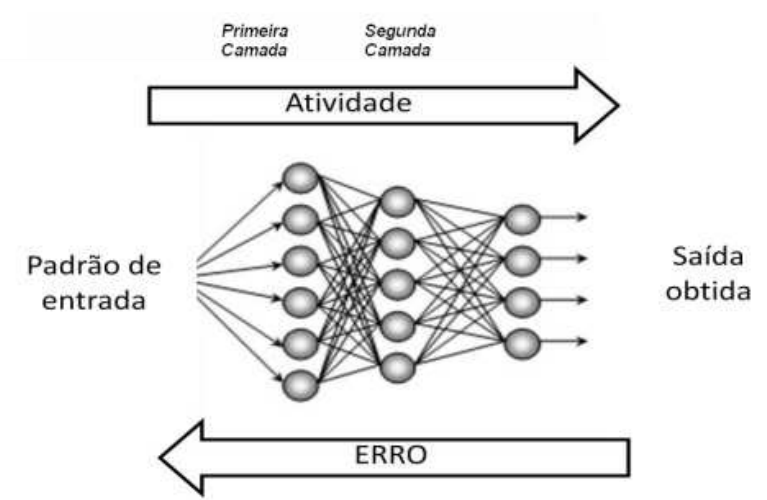
\includegraphics[width=\linewidth]{figuras/MLP/atividade_MLP.png}
      \caption{\textit{Forward} e \textit{backward} em uma rede MLP.}
      \label{fig:subfigura2}
    \end{subfigure}
    \label{fig:subfiguras}
  \end{figure}

\section{Naive Bayes}

Naive Bayes um método de classificação e tem como base o teorema de Bayes. Este método
gera uma tabela de probabilidades utilizadas para classificar os dados, as features dos 
dados são analisadas de forma independente, por isso o nome \textit{Naive}, que significa
ingênuo.

\begin{itemize}
    \item Teorema de Bayes:
    \begin{equation}
        P(y|x) = P(y)P(x|y)/P(x)
        \label{eq:mass_energy_equation}
    \end{equation}

\end{itemize}
% \item 



\section{SVM com kernel RBF}



\section{SVM com kernel Polinomial}

\section{SVM com kernel Linear}
